\chapter{Test Strategy, Results and Analysis}
\section{Test strategy}
At the beginning of the testing phase of the thesis, both applications are given the same amount of memory to ensure they have the same CPU share. It turns out, Java has nearly twice much throughput as the Node.js application. It seems one is comparing something which is totally not comparable at all. It is also quite far away from expectation. Things are tried and investigations are made to identify the cause. \\
The monitoring on CPU usage shows that the Java application can utilize up to 250\%,  in contrast which the Node.js application never quite exceeds the limit of 100\%. This has everything to do with the single-threaded principle of Node.js applications. While Java application is through adding CPU and memory vertical scalable, Node.js is single-threaded and scales by creating multiple-node processes. It is only fair to test both application when they utilize the same amount of CPUs. However, the Cloud Foundry specific way of designating computing resources ensures there is no neat cut of a piece of CPU unless one is completely alone in the land scape. Therefore, multiple configuration of tests are conducted and described in this chapter so one can analyze the results from different aspects.  \\

\section{Test with optimal response time}
In this test, fixed variable is average end-to-end response time which is kept under 10 ms  as a criteria for optimal performance. An additional bar is set on the CPU consumption which can not exceed 100\%. \\
In the context of Cloud Foundry, it is impossible to assure an application using only one core. Setting the memory of application can limit the CPU shares it can get. Nevertheless, if other applications on the same node are idling, even the tiniest application can get all the 4 CPUs of the node. In terms of Java application, it is already much more memory consuming than node as shown in \ref{memory} hence it is highly unlikely only one CPU is given to the application. What one witnesses as a 70\% CPU is also very likely distributed in several CPUs.\\
Figure\ref{cpu-100} shows the result of the test described above. It can be deducted from the graph, that Java has a better performance in comparison with Node.js. As the CPU distribution is unclear,  it can be accounted for that Java application is likely running with 4 or 2 very relaxed CPUs while Node.js is grabbing every bit of computing resource from that single CPU. This also leads to the reflection on the results of benchmarking from TechPower \citep{benchmark}. In terms of applications on cloud, Java is twice more efficient than Node.js. It is possible they haven't taken the CPU distribution into consideration. 

\begin{figure}[h]
	\centering
	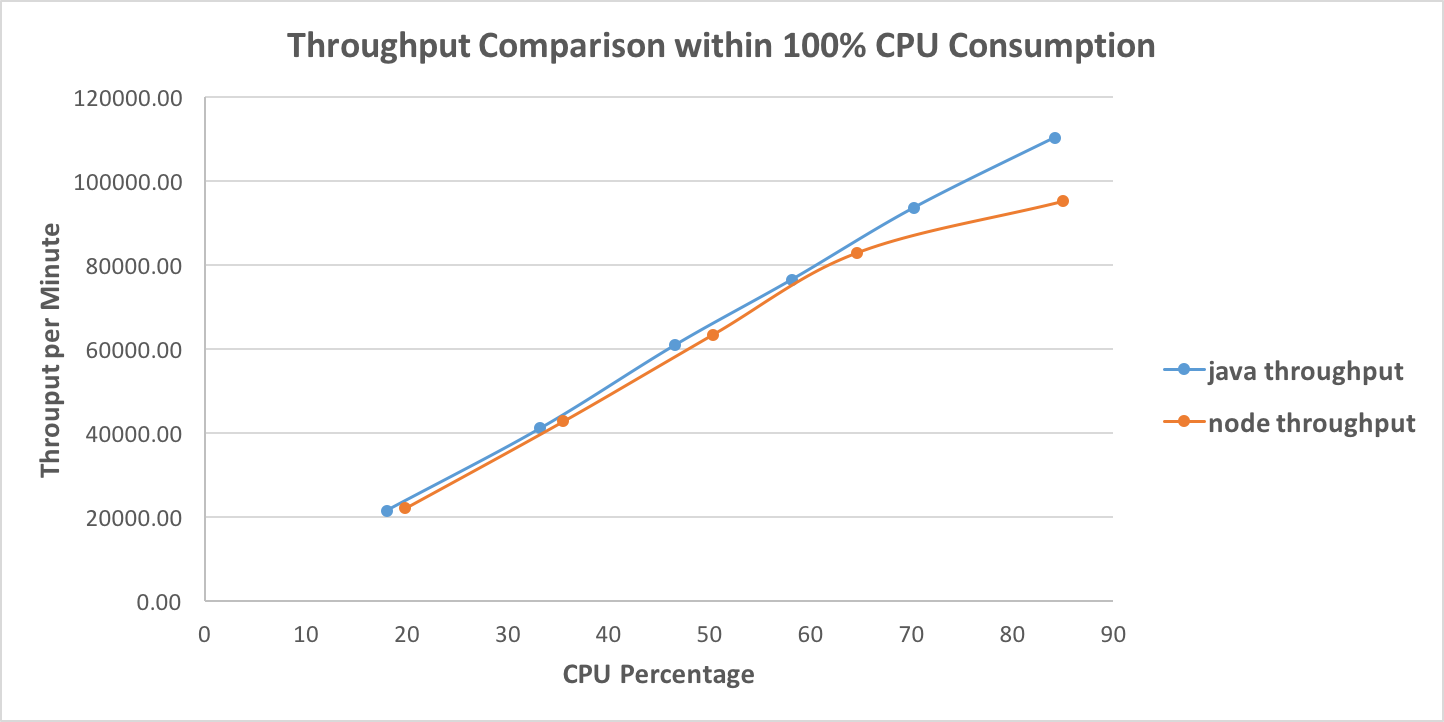
\includegraphics[width=10cm]{cpu-100}
	\caption{Compare throughput under 100 CPU consumption}
	\label{cpu-100}
\end{figure}


\section{Test with real load}
\subsection{Test configuration}
 In this round of test, applications are going to scale. Then how should it be contemplated whether two applications are equally scaled? As found out earlier, one Java instance utilizes more CPU while one Node.js employs only one, which leads the test to comparing vertical scaling in Java application with horizontal scaling in Node.js. This is still feasible if one can be sure Java always obtains the same CPUs. However, figure \ref{java-cpu-limit} shows, that Java application never get to use all of its 4 CPUs. The database connection and router load are checked and they are not under stress at all.  An abnormal increase in memory is observed which indicates something suspicious in the application. The implementation is scrutinized, nevertheless, in the thesis no obvious cause is found. This leads to the realization that even though one Java instance gains 4 CPUs, it doesn't equal to four one-CPU Node instances because somehow not all 4 CPUs are put in use. 
 
 \begin{figure}[h]
 	\centering
 	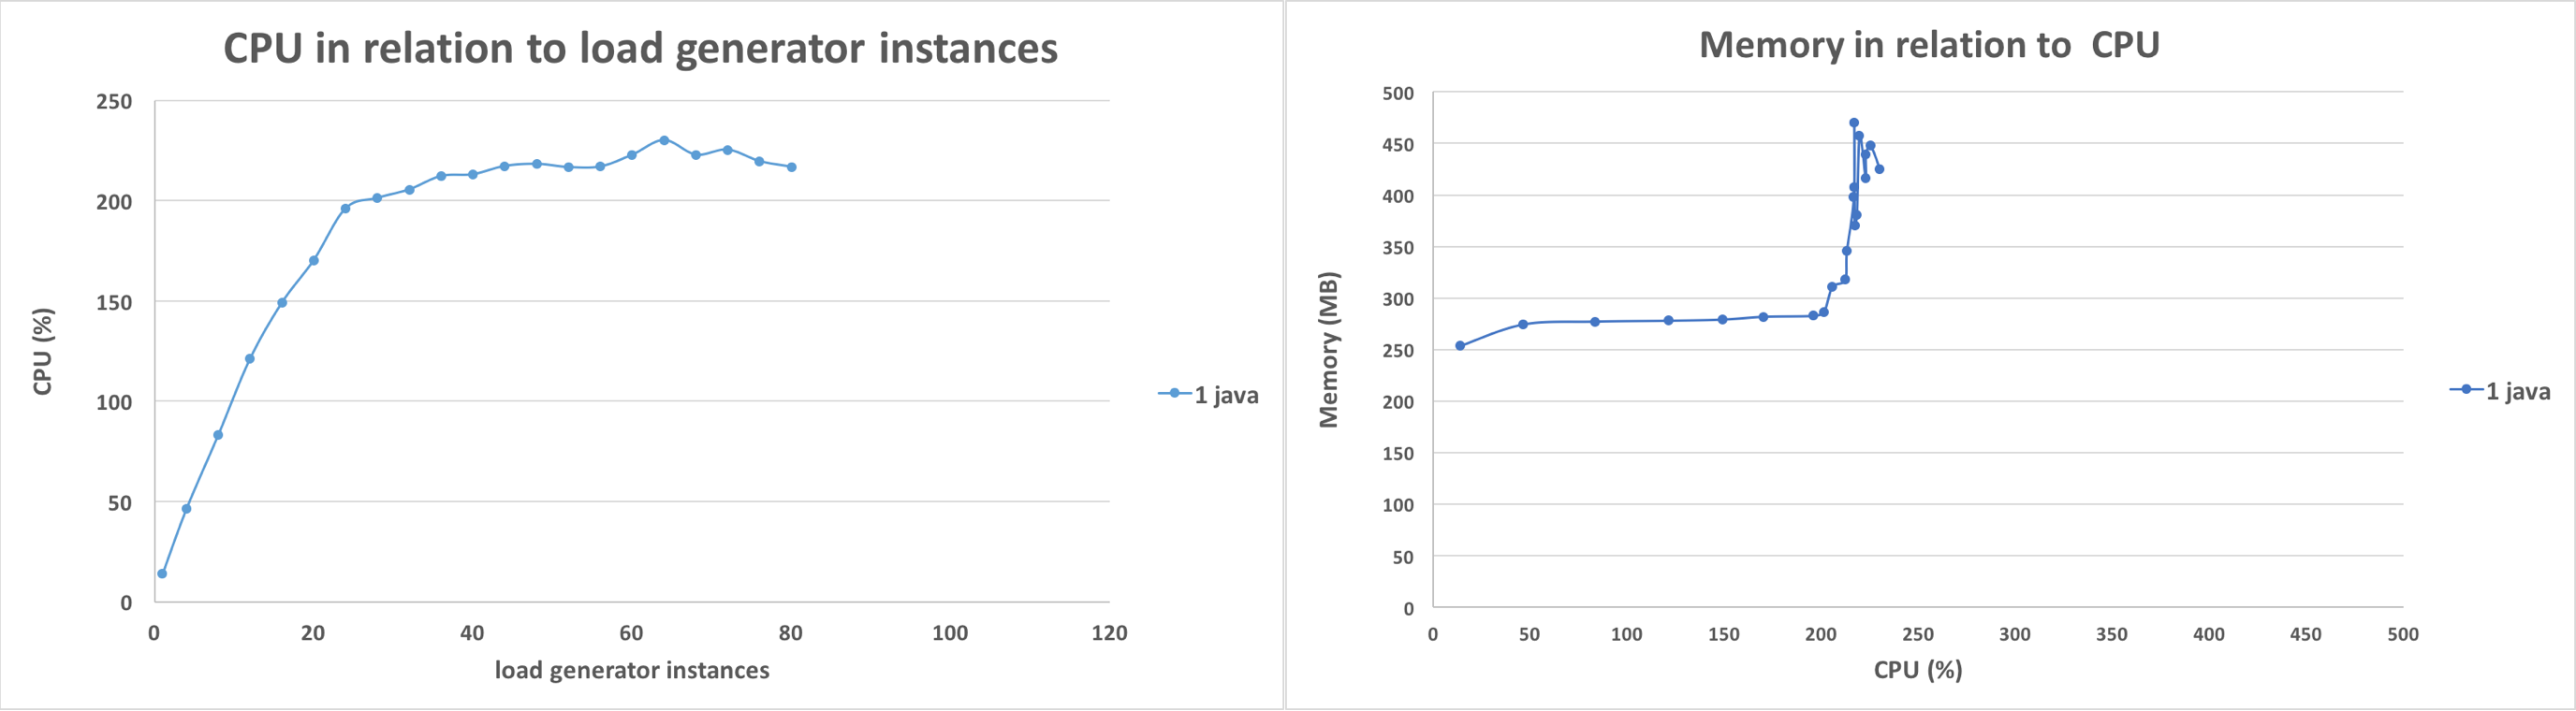
\includegraphics[width=10cm]{java-cpu-limit}
 	\caption{Limited CPU usage in Java application}
 	\label{java-cpu-limit}
 \end{figure}
Therefore the comparison in the thesis would not restricted to one Java instance against some multiple instances from Node.js. Load will be continuously added on to the application. Then the applications will scale when the response time shows a clear tendency to climb. At the end, an aggregated comparison will be made in terms of scalability in respect to CPU and instance. \\
Load is brought about through sending one request on application per instance of load generator.It is decided not to send parallel requests so as to guarantee each instance of the generator is simulating one end user. With each new round of test, 4 instances will be added to the existing running load generator. The maximum load generator instances will be 96 so that the limitation of database connection pool size will not be exceeded.\\
Java application will stop scaling when router has reached its limit (70\% load). For Node.js applications, the scaling stops when the CPU usage reaches the maximum CPU usage of Java applications tested previously.
 
\subsection{Test result}
 \begin{figure}[h]
	\centering
	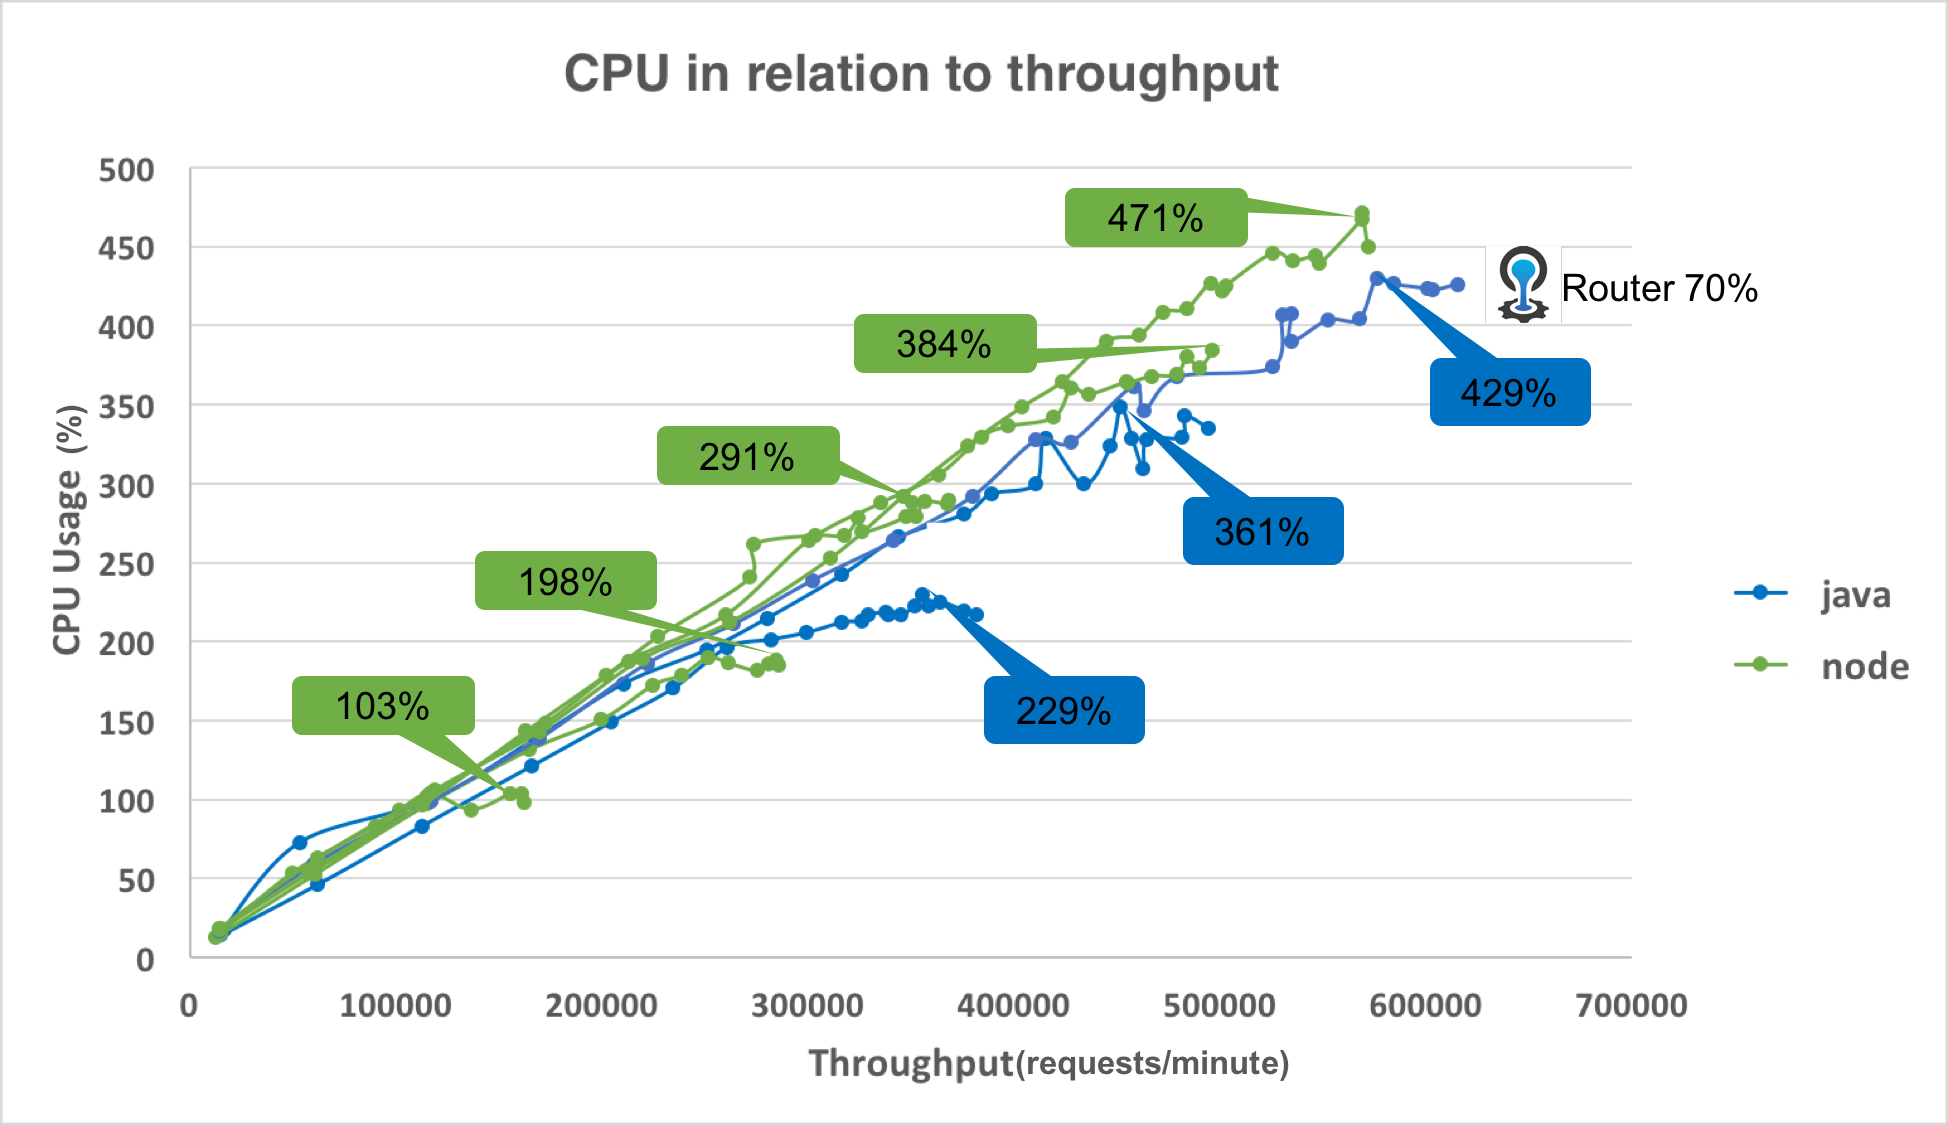
\includegraphics[width=10cm]{all-app-cpu}
	\caption{Throughput in relation to CPU}
	\label{all-app-cpu}
\end{figure}
In figure \ref{all-app-cpu}, it is illustrated the throughput in relation to the CPU usage of Java application in running instance numbers of 1, 2, and 3. The xx axis is the throughput , the yy axis is the CPU consumption. When 3 Java applications are running, the router reaches its maximum capacity and becomes bottleneck because no more requests can be handled without losing time spent waiting for the load balancing in router. As summarized in table \ref{app-cpu-usage}, with every increase of instance, the CPU usage from total available CPU decreases, which indicates the application doesn't scale horizontally by adding more instances. 
\begin{table}[h]
	\caption{Percentage of utilized CPU}
	\label{app-cpu-usage}
	\renewcommand{\arraystretch}{1.2}
	\centering
	\sffamily
	\begin{footnotesize}
		\begin{tabular}{l l l l l  }
			\toprule
			\textbf{Application  type} &\textbf{Instance Number} & \textbf{Available CPU \%} & \textbf{Maximum CPU\%}& \textbf{Utilzed CPU} }\\
		\midrule
		Java &1 	&	229	 & 400 & 57\% \\
		Java &2	&	361 & 800& 45\% \\
		Java &3	&	429  &	1200 & 35\%\\
				\midrule
			Node.js &1 	&	103	 & 100 & 103\% \\
		Node.js &2	&	198 &  200& 99\% \\
		Node.js &3	&	291 & 300 & 97\%\\
		Node.js &4	&	384 & 400 & 96\%\\
		Node.js &5	&	471 & 500 & 94\%\\
		\bottomrule
	\end{tabular}
\end{footnotesize}
\rmfamily
\end{table}

The same performance information of Node.js application is also depicted in figure \ref{all-app-cpu}. The test ends with 5 instances of Node.js application , which is when the CPU usage is in the same range of Java one. As summarized in table \ref{app-cpu-usage}, application shows a quite steady utilization of more than 90\% of the available CPU resources. It implies a horizontal scaling towards adding instances. If we draw a line down to the xx axis to see the correspondent throughput like \ref{cpu-node}, we can see the throughput scales also with adding instances. Since every instance make full use of the CPU, the throughput scales also linear per CPU. \\
 \begin{figure}[h]
	\centering
	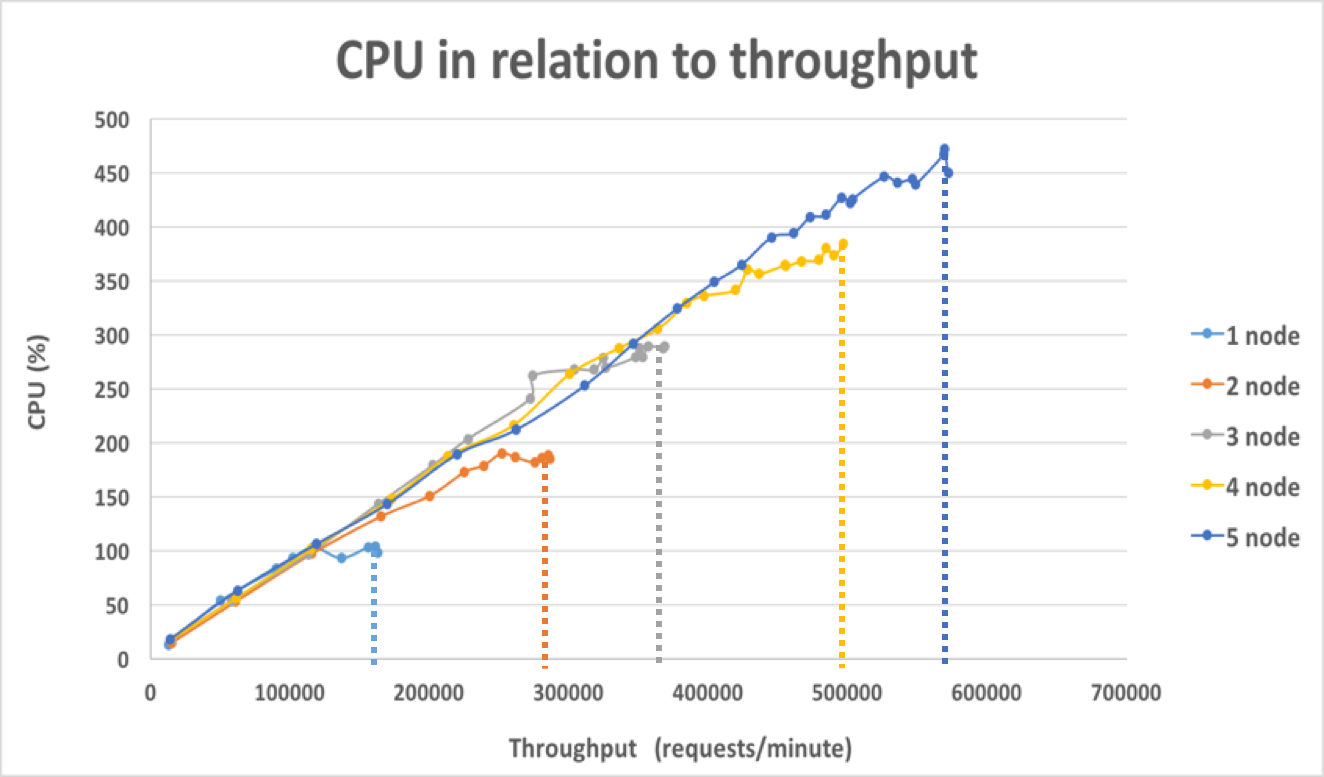
\includegraphics[width=10cm]{cpu-node}
	\caption{cpu efficiency of Node.js application}
	\label{cpu-node}
\end{figure}

Although we observe an inefficient utilization of available CPU from Java application, we still want to know whether the applied computing resource is efficiently used. Figure \ref{cpu-java} presents the same relation between CPU and throughput from a Java application with 3 running instances. Here we can have a look how the throughput scales when more CPU is given to a Java application. We can see the throughput scales almost linear with more CPUs.
 \begin{figure}[h]
	\centering
	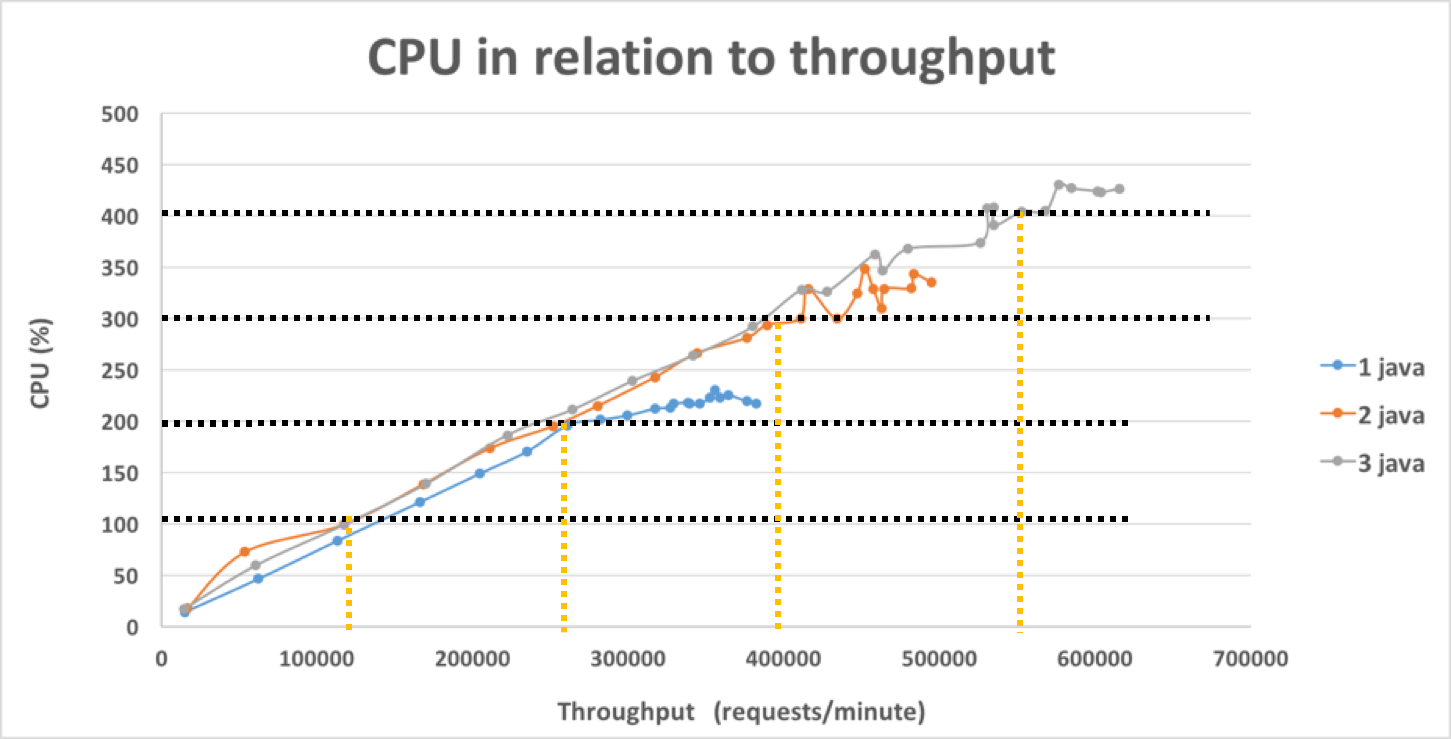
\includegraphics[width=10cm]{cpu-java}
	\caption{cpu efficiency of 3 Java instances}
	\label{cpu-java}
\end{figure}

The last metric to check is memory consumption. As displayed in figure \ref{all-app-memory}, Node.js shows excellent memory utilization for the whole test range while Java is quite memory demanding. Although it offers some performance gains in terms of handling more requests than the Node.js, it is not in proportion with the memory consumption. \\

 \begin{figure}[h]
	\centering
	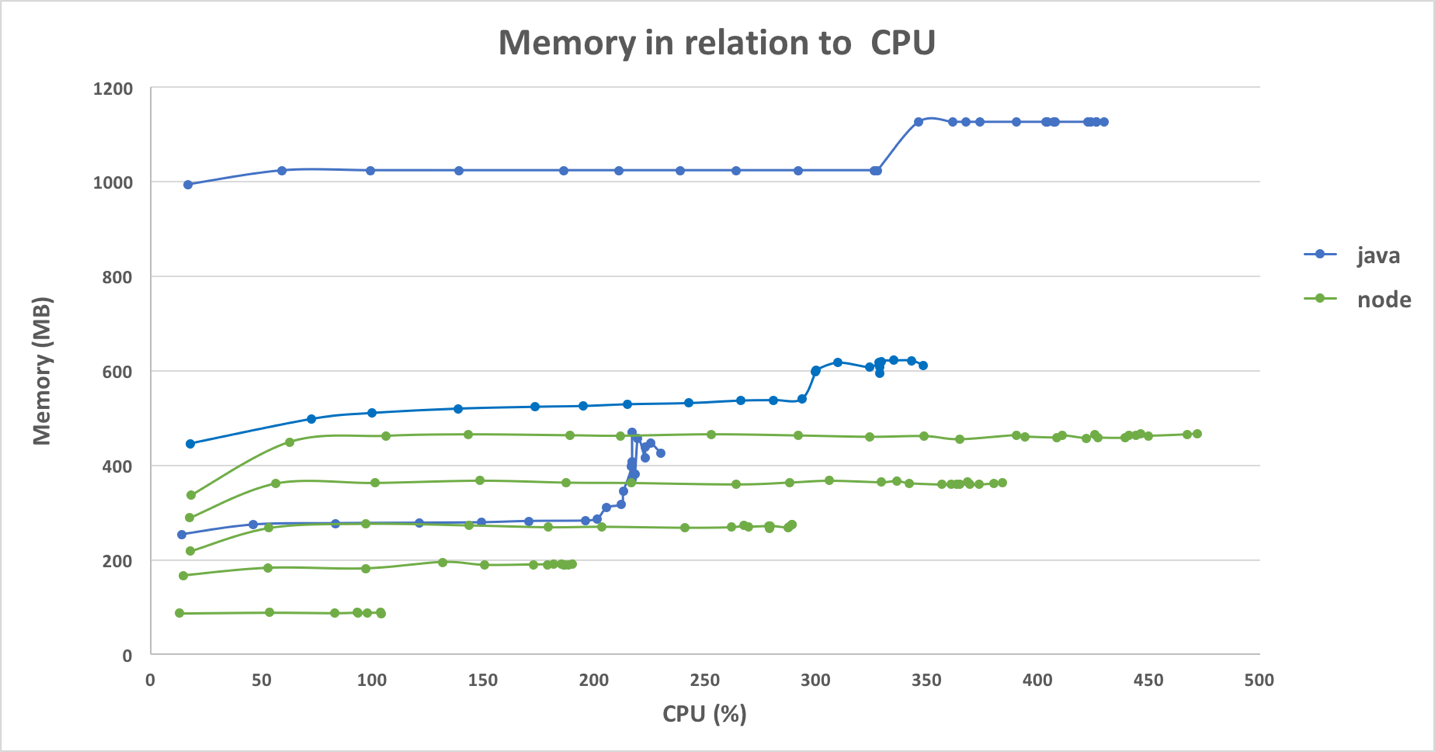
\includegraphics[width=10cm]{all-app-mem}
	\caption{Memory in relation to throughput}
	\label{all-app-memory}
\end{figure}

However, another abnormality in the sudden surge in the case of one Java instance should acquire our attention. This might reveal some cause for the incapability of using all the CPU power assigned to the application. If the memory consumption fluctuation and inefficient CPU utilization can be resolved,  Java would demonstrate a great vertical scalability. Although Node.js needs less memory for a single instance, the horizontal scaling requires the memory consumption to multiply itself. In the end, one Java instance which make full use of 12 CPUs would be much more memory efficient that 12 small Node.js instances. 